\section{Walk}
\subsection*{题意}
给定一个 $n$ 个点的有向图,求图中有多少条长度为 $k$ 的路径。

注:路径可以经过同一顶点和边。
\subsection*{样例}
\begin{center}
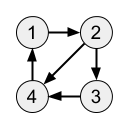
\includegraphics[width=3cm]{./Pics/R.png}

\end{center}
\begin{center}
一共有 $6$ 条长度为 $2$ 的路径:
\begin{itemize}
\item \begin{center}1 → 2 → 3\end{center}
\item \begin{center}1 → 2 → 4\end{center}
\item \begin{center}2 → 3 → 4\end{center}
\item \begin{center}2 → 4 → 1\end{center}
\item \begin{center}3 → 4 → 1\end{center}
\item \begin{center}4 → 1 → 2\end{center}
\end{itemize}
\end{center}
\subsection*{数据范围}
\begin{itemize}
\item $1 \leq n \leq 50$
\item $1 \leq k \leq 10^{18}$
\end{itemize}


\subsection*{题解}

我们设 $\texttt{dp}[n][i][j]$ 表示起点和终点分别是 $i$ 和 $j$,一共走了 $n$ 步的方案数。 

Base case 是简单的,$\texttt{dp}[1][i][j]$ 就等于有多少条从 $i$ 到 $j$ 的有向边。

转移方程很显然,我们只需要枚举上一步的位置$k$ 即可:
$$
\texttt{dp}[n+1][i][j] = \sum_{k = 1}^n \texttt{dp}[n][i][k] \times \texttt{dp}[1][k][j] 
$$

朴素计算的复杂度是 $O(kn^3)$,在$k$高达$10^{18}$的情况下无法通过。

注意到上述方法本质是:
$$
\text{走n+1步} = \text{走n步} + \text{走1步}
$$

但我们当然可以拆得更多:

\begin{enumerate}
    \item $\text{走2n步} = \text{走n步} + \text{走n步}$
    \item $\text{走2n+1步} = \text{走2n步} + \text{走1步}$
\end{enumerate}

其实也就是利用快速幂的思想,只不过这里变成了矩阵的幂。由于每走两步,$k$至少下降一半,复杂度变为 $O(\log(k)n^3)$,可以通过。具体实现参考代码。


\subsection*{核心代码}
\inputminted[linenos,autogobble]{cpp}{./Code/R.cpp}
\newpage